% Options for packages loaded elsewhere
\PassOptionsToPackage{unicode}{hyperref}
\PassOptionsToPackage{hyphens}{url}
\PassOptionsToPackage{dvipsnames,svgnames*,x11names*}{xcolor}
%
\documentclass[
]{book}
\usepackage{lmodern}
\usepackage{amssymb,amsmath}
\usepackage{ifxetex,ifluatex}
\ifnum 0\ifxetex 1\fi\ifluatex 1\fi=0 % if pdftex
  \usepackage[T1]{fontenc}
  \usepackage[utf8]{inputenc}
  \usepackage{textcomp} % provide euro and other symbols
\else % if luatex or xetex
  \usepackage{unicode-math}
  \defaultfontfeatures{Scale=MatchLowercase}
  \defaultfontfeatures[\rmfamily]{Ligatures=TeX,Scale=1}
\fi
% Use upquote if available, for straight quotes in verbatim environments
\IfFileExists{upquote.sty}{\usepackage{upquote}}{}
\IfFileExists{microtype.sty}{% use microtype if available
  \usepackage[]{microtype}
  \UseMicrotypeSet[protrusion]{basicmath} % disable protrusion for tt fonts
}{}
\makeatletter
\@ifundefined{KOMAClassName}{% if non-KOMA class
  \IfFileExists{parskip.sty}{%
    \usepackage{parskip}
  }{% else
    \setlength{\parindent}{0pt}
    \setlength{\parskip}{6pt plus 2pt minus 1pt}}
}{% if KOMA class
  \KOMAoptions{parskip=half}}
\makeatother
\usepackage{xcolor}
\IfFileExists{xurl.sty}{\usepackage{xurl}}{} % add URL line breaks if available
\IfFileExists{bookmark.sty}{\usepackage{bookmark}}{\usepackage{hyperref}}
\hypersetup{
  pdftitle={Introductory Mathematics for Economists with Matlab},
  pdfauthor={Priuz Saboury and Fan Wang},
  colorlinks=true,
  linkcolor=Maroon,
  filecolor=Maroon,
  citecolor=Blue,
  urlcolor=blue,
  pdfcreator={LaTeX via pandoc}}
\urlstyle{same} % disable monospaced font for URLs
\usepackage{longtable,booktabs}
% Correct order of tables after \paragraph or \subparagraph
\usepackage{etoolbox}
\makeatletter
\patchcmd\longtable{\par}{\if@noskipsec\mbox{}\fi\par}{}{}
\makeatother
% Allow footnotes in longtable head/foot
\IfFileExists{footnotehyper.sty}{\usepackage{footnotehyper}}{\usepackage{footnote}}
\makesavenoteenv{longtable}
\usepackage{graphicx,grffile}
\makeatletter
\def\maxwidth{\ifdim\Gin@nat@width>\linewidth\linewidth\else\Gin@nat@width\fi}
\def\maxheight{\ifdim\Gin@nat@height>\textheight\textheight\else\Gin@nat@height\fi}
\makeatother
% Scale images if necessary, so that they will not overflow the page
% margins by default, and it is still possible to overwrite the defaults
% using explicit options in \includegraphics[width, height, ...]{}
\setkeys{Gin}{width=\maxwidth,height=\maxheight,keepaspectratio}
% Set default figure placement to htbp
\makeatletter
\def\fps@figure{htbp}
\makeatother
\setlength{\emergencystretch}{3em} % prevent overfull lines
\providecommand{\tightlist}{%
  \setlength{\itemsep}{0pt}\setlength{\parskip}{0pt}}
\setcounter{secnumdepth}{5}
\usepackage{bbm}
\usepackage{booktabs}
\usepackage{longtable}
\usepackage{array}
\usepackage{multirow}
\usepackage{wrapfig}
\usepackage{float}
% \floatplacement{figure}{H}
\usepackage[labelformat = empty]{caption}
\usepackage{colortbl}
\usepackage{pdflscape}
\usepackage{tabu}
\usepackage{threeparttable}
\usepackage{threeparttablex}
\usepackage[normalem]{ulem}
\usepackage{makecell}
\usepackage{xcolor}
\usepackage{geometry}
\geometry{
	a4paper,
	left=1.0in,
	right=1.0in,
	top=1.0in,
	bottom=1.0in,
}
\setcounter{secnumdepth}{5}
\setcounter{tocdepth}{5}
\usepackage[]{natbib}
\bibliographystyle{apalike}

\title{Introductory Mathematics for Economists with Matlab}
\author{Priuz Saboury and Fan Wang}
\date{2023-01-24}

\begin{document}
\maketitle

{
\hypersetup{linkcolor=}
\setcounter{tocdepth}{1}
\tableofcontents
}
\hypertarget{preface}{%
\chapter*{Preface}\label{preface}}
\addcontentsline{toc}{chapter}{Preface}

This is a work-in-progress \href{http://math4econ.github.io/}{course website} for Mathematics for Economists, an upper-level undergraduate economics course offered by \href{https://piruzsaboury.weebly.com/}{Piruz Saboury} and \href{https://fanwangecon.github.io/}{Fan Wang}. The course covers a subset of topics from \emph{Mathematics for Economists} \citep{simonblume1994}. Applications focus on households' optimal borrowing and savings problems and firms' optimal inputs problems. Matlab is used throughout.

\begin{quote}
\href{https://Math4Econ.github.io/bookdown}{\textbf{bookdown site}} and \href{https://Math4econ.github.io/bookdown/Introductory-Mathematics-for-Economists-with-Matlab.pdf}{\textbf{bookdown pdf}}.
\end{quote}

Materials are written in \href{https://www.mathworks.com/products/matlab.html}{matlab} \citep{matlab} livescript files and shown as HTML files. For HTML files, click on the links below. The livescript files can be downloaded and modified inside matlab. Files are from the \href{https://github.com/Math4Econ/Math4Econ.github.io}{Math4Econ} repository.

Please contact \href{https://piruzsaboury.weebly.com/}{Piruz Saboury} or \href{https://fanwangecon.github.io/}{Fan Wang} for issues or problems.

From other repositories: for research support toolboxes, see \href{https://fanwangecon.github.io/mecontools/}{matlab toolbox}, \href{https://fanwangecon.github.io/recontools/}{r toolbox}, and \href{https://pyfan.readthedocs.io/en/latest/}{python toolbox}; for code examples, see \href{https://fanwangecon.github.io/m4econ/}{matlab examples}, \href{https://fanwangecon.github.io/stata4econ/}{stata examples}, \href{https://fanwangecon.github.io/r4econ/}{r examples}, \href{https://fanwangecon.github.io/py4econ/}{python examples}, and \href{https://fanwangecon.github.io/tex4econ/}{latex examples}; for packaging example, see \href{http://fanwangecon.github.io/pkgtestr}{pkgtestr} for developing r packages; for teaching, also see \href{https://fanwangecon.github.io/stat4econ/}{intro statistics for undergraduates}.

The site is built using \href{https://bookdown.org/}{Bookdown} \citep{R-bookdown}.

\hypertarget{notations-and-functions}{%
\chapter{Notations and Functions}\label{notations-and-functions}}

\hypertarget{local-and-global-maximum}{%
\section{Local and Global Maximum}\label{local-and-global-maximum}}

\begin{quote}
Go back to \href{https://math4econ.github.io/}{Introductory Mathematics for Economists with Matlab} (\href{https://math4econ.github.io/bookdown}{bookdown site}). Also see \href{http://fanwangecon.github.io/M4Econ}{M4Econ} and \href{https://fanwangecon.github.io/MEconTools/}{MEconTools}.
\end{quote}

\textbf{Definition}

\begin{itemize}
\item
  \textbf{Global Maximum:} Function \(f\) defined on domain \(X\) has a
  \textbf{global} maximum at \(x^* \in X\) if for all \(x\in X\),
  \(f(x)\le f(x^* )\)
\item
  \textbf{Local Maximum:} Function \(f\) defined on domain \(X\) has a
  \textbf{local} maximum at \(x^* \in X\) if there exists an open interval
  \(\left(a,b\right)\), such that \(x^* \in \left(a,b\right)\), and for
  all \(x\in \left(a,b\right)\), \(f(x)\le f(x^* )\)
\end{itemize}

It should be noted that Many functions do not have maximum. We have
utility function, production function, and budget constraints (and other
functions) in economic models. When households make utility maximizing
choices, they pick the bundle of goods that gives them the highest level
of utility. Many of the production and utility functions that we use do
not have local or global maximum. For example, a Cobb-Douglas production
function will produce ever higher output with more labor and capital
input. And a log utility function will give higher utility with higher
levels of consumption. When we combine preference and budget together,
we could think about the optimal bundle of choices that achieves the
highest level of utility given fixed budget in a household maximization
problem.

\textbf{Quadratic Utility}

A special utility function, quadratic utility, however, does have a
single maximum.

\[U(x)=x-\alpha \cdot x^2\]

We can write down the equation using matlab's symbolic package

\begin{verbatim}
% Parameter
a = 0.20;
% Create symbolic equation in matlab
syms x
f(x) = x - a*x^2
\end{verbatim}

f(x) =

\(\displaystyle x-\frac{x^2 }{5}\)

\textbf{Matlab Analytical Global Maximum for Quadratic Utility}

Matlab can find the \(x\) value that maximizes the function by using the
following functions from its symbolic toolbox:

\begin{itemize}
\item
  \textbf{diff} function: taking the derivative of f with respect to \(x\)
\item
  \textbf{solve} function: finding where the derivative crosses \(0\)
\end{itemize}

\begin{verbatim}
% Solve
maxofx = solve(diff(f, x), x)
\end{verbatim}

maxofx =

\(\displaystyle \frac{5}{2}\)

\begin{verbatim}
% Convert symbolic to double precision
maxofx = double(maxofx)

maxofx = 2.5000
\end{verbatim}

We have found the global maximum for the function.

A household will try to consume exactly this optimal amount of good if
their budget allows.

With quadratic utility over one good, even if the household can afford
to buy more goods than the maximum amount, they will not.

This could be used to approximate consumption of say how much rice a
consumer wants for example.

\textbf{Matlab Graphical Solution}

\begin{verbatim}
% Graph equation
close all;
figure();
% Create minimum x and maximum x point where to draw the graph
x_lower_bd = min(-10, maxofx-abs(maxofx)/2);
x_upper_bd = max(10, maxofx+abs(maxofx)/2);
% Draw the function
fplot(f, [x_lower_bd, x_upper_bd]);
% Label
xlabel(['X-axis, Quadratic Utility, max U reached at x=', num2str(maxofx)])
ylabel(['Utility'])
grid on
\end{verbatim}

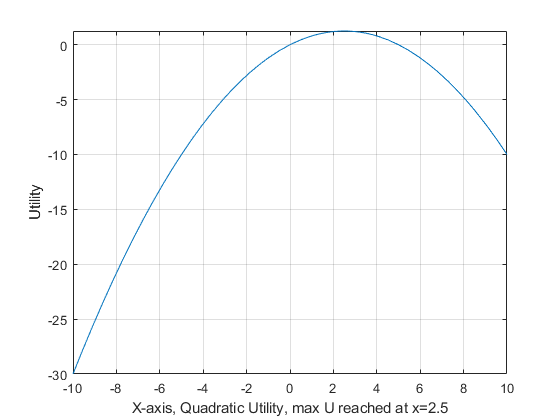
\includegraphics[width=5.20833in,height=\textheight]{img/localglobal_images/figure_0.png}

\hypertarget{appendix-appendix}{%
\appendix}


\hypertarget{index-and-code-links}{%
\chapter{Index and Code Links}\label{index-and-code-links}}

\hypertarget{notations-and-functions-links}{%
\section{Notations and Functions links}\label{notations-and-functions-links}}

\begin{enumerate}
\def\labelenumi{\arabic{enumi}.}
\tightlist
\item
  \href{https://Math4Econ.github.io/calconevar/htmlpdfm/localglobal.html}{Local and Global Maximum}: \href{https://github.com/Math4Econ/Math4Econ.github.io/blob/main/calconevar/localglobal.mlx}{\textbf{mlx}} \textbar{} \href{https://github.com/Math4Econ/Math4Econ.github.io/blob/main/calconevar/htmlpdfm/localglobal.m}{\textbf{m}} \textbar{} \href{https://github.com/Math4Econ/Math4Econ.github.io/blob/main/calconevar/htmlpdfm/localglobal.pdf}{\textbf{pdf}} \textbar{} \href{https://Math4Econ.github.io/calconevar/htmlpdfm/localglobal.html}{\textbf{html}}

  \begin{itemize}
  \tightlist
  \item
    local and global maximum.
  \item
    \textbf{m}: \emph{syms + solve() + diff() + double() + double(solve(diff(f,x),x)), fplot(f,{[}x\_low, x\_high{]})}
  \end{itemize}
\end{enumerate}

  \bibliography{book.bib,packages.bib}

\end{document}
